% !TEX encoding = UTF-8 Unicode
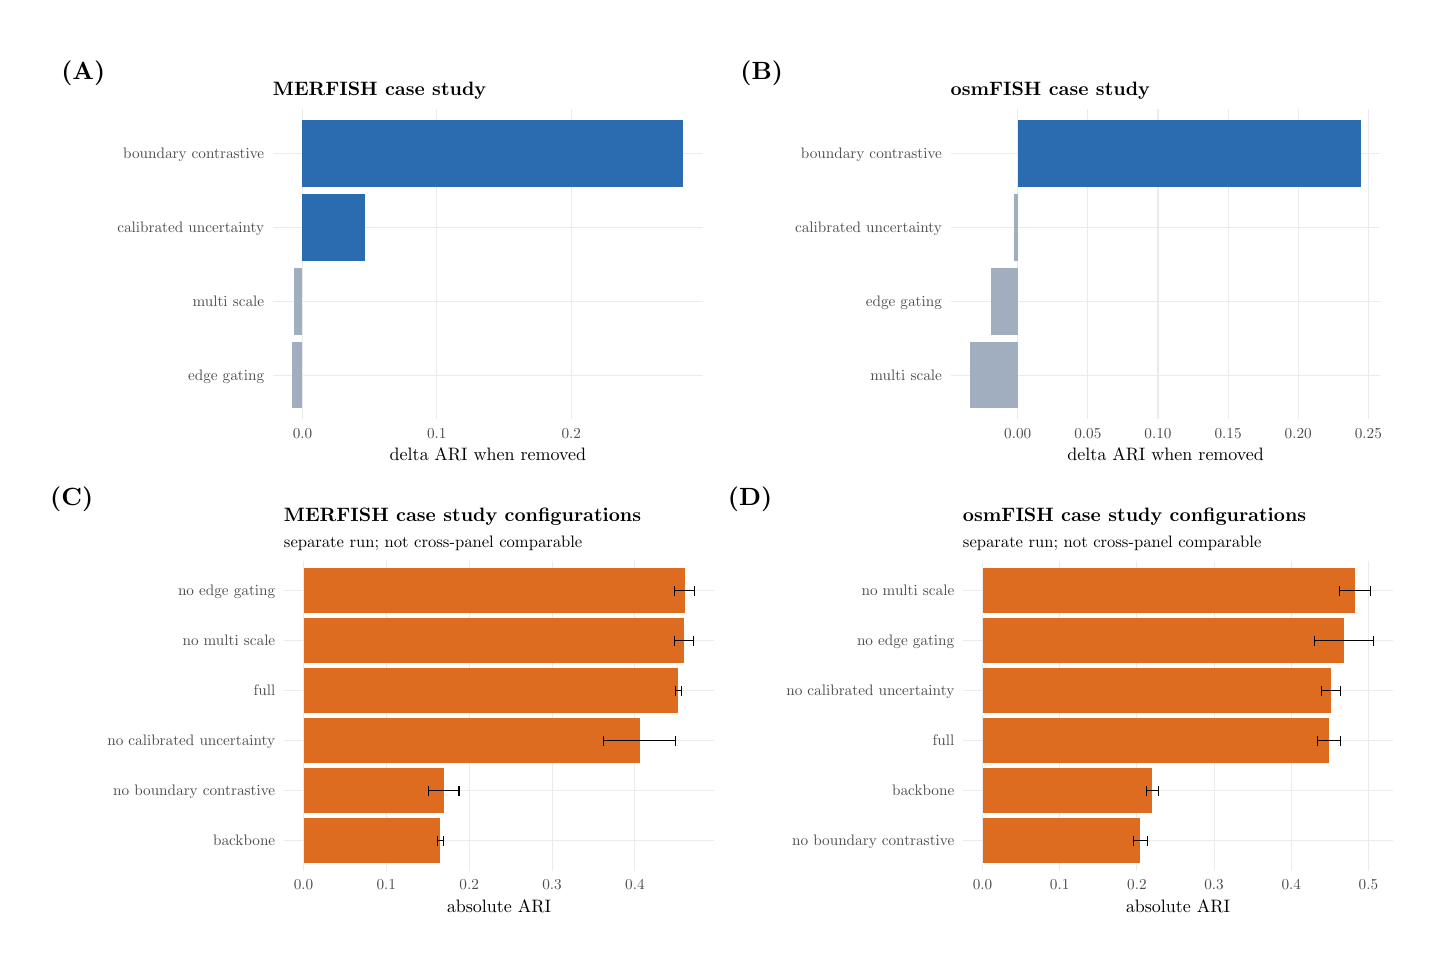
\begin{tikzpicture}[x=1pt,y=1pt]
\definecolor{fillColor}{RGB}{255,255,255}
\path[use as bounding box,fill=fillColor,fill opacity=0.00] (0,0) rectangle (501.28,328.16);
\begin{scope}
\path[clip] (  0.00,  0.00) rectangle (501.28,328.16);
\definecolor{drawColor}{RGB}{255,255,255}
\definecolor{fillColor}{RGB}{255,255,255}

\path[draw=drawColor,line width= 0.6pt,line join=round,line cap=round,fill=fillColor] (  0.00,  0.00) rectangle (501.28,328.16);
\end{scope}
\begin{scope}
\path[clip] (  5.50,164.08) rectangle (250.64,322.66);
\definecolor{drawColor}{RGB}{255,255,255}
\definecolor{fillColor}{RGB}{255,255,255}

\path[draw=drawColor,line width= 0.6pt,line join=round,line cap=round,fill=fillColor] (  5.50,164.08) rectangle (250.64,322.66);
\end{scope}
\begin{scope}
\path[clip] (250.64,164.08) rectangle (495.78,322.66);
\definecolor{drawColor}{RGB}{255,255,255}
\definecolor{fillColor}{RGB}{255,255,255}

\path[draw=drawColor,line width= 0.6pt,line join=round,line cap=round,fill=fillColor] (250.64,164.08) rectangle (495.78,322.66);
\end{scope}
\begin{scope}
\path[clip] (  8.16,167.04) rectangle (247.98,319.70);
\definecolor{fillColor}{RGB}{255,255,255}

\path[fill=fillColor] (  8.16,167.04) rectangle (247.98,319.70);
\end{scope}
\begin{scope}
\path[clip] ( 88.60,186.61) rectangle (243.98,298.63);
\definecolor{drawColor}{gray}{0.92}

\path[draw=drawColor,line width= 0.4pt,line join=round] ( 88.60,202.61) --
	(243.98,202.61);

\path[draw=drawColor,line width= 0.4pt,line join=round] ( 88.60,229.28) --
	(243.98,229.28);

\path[draw=drawColor,line width= 0.4pt,line join=round] ( 88.60,255.95) --
	(243.98,255.95);

\path[draw=drawColor,line width= 0.4pt,line join=round] ( 88.60,282.62) --
	(243.98,282.62);

\path[draw=drawColor,line width= 0.4pt,line join=round] ( 99.30,186.61) --
	( 99.30,298.63);

\path[draw=drawColor,line width= 0.4pt,line join=round] (147.86,186.61) --
	(147.86,298.63);

\path[draw=drawColor,line width= 0.4pt,line join=round] (196.42,186.61) --
	(196.42,298.63);
\definecolor{fillColor}{RGB}{43,108,176}

\path[fill=fillColor] ( 99.30,270.62) rectangle (236.92,294.62);

\path[fill=fillColor] ( 99.30,243.95) rectangle (121.98,267.95);
\definecolor{fillColor}{RGB}{160,174,192}

\path[fill=fillColor] ( 95.66,190.61) rectangle ( 99.30,214.61);

\path[fill=fillColor] ( 96.25,217.28) rectangle ( 99.30,241.28);
\end{scope}
\begin{scope}
\path[clip] (  0.00,  0.00) rectangle (501.28,328.16);
\definecolor{drawColor}{gray}{0.30}

\node[text=drawColor,anchor=base east,inner sep=0pt, outer sep=0pt, scale=  0.55] at ( 85.45,200.72) {edge gating};

\node[text=drawColor,anchor=base east,inner sep=0pt, outer sep=0pt, scale=  0.55] at ( 85.45,227.39) {multi scale};

\node[text=drawColor,anchor=base east,inner sep=0pt, outer sep=0pt, scale=  0.55] at ( 85.45,254.06) {calibrated uncertainty};

\node[text=drawColor,anchor=base east,inner sep=0pt, outer sep=0pt, scale=  0.55] at ( 85.45,280.73) {boundary contrastive};
\end{scope}
\begin{scope}
\path[clip] (  0.00,  0.00) rectangle (501.28,328.16);
\definecolor{drawColor}{gray}{0.30}

\node[text=drawColor,anchor=base,inner sep=0pt, outer sep=0pt, scale=  0.55] at ( 99.30,179.67) {0.0};

\node[text=drawColor,anchor=base,inner sep=0pt, outer sep=0pt, scale=  0.55] at (147.86,179.67) {0.1};

\node[text=drawColor,anchor=base,inner sep=0pt, outer sep=0pt, scale=  0.55] at (196.42,179.67) {0.2};
\end{scope}
\begin{scope}
\path[clip] (  0.00,  0.00) rectangle (501.28,328.16);
\definecolor{drawColor}{RGB}{0,0,0}

\node[text=drawColor,anchor=base,inner sep=0pt, outer sep=0pt, scale=  0.65] at (166.29,171.58) {delta ARI when removed};
\end{scope}
\begin{scope}
\path[clip] (  0.00,  0.00) rectangle (501.28,328.16);
\definecolor{drawColor}{RGB}{0,0,0}

\node[text=drawColor,anchor=base west,inner sep=0pt, outer sep=0pt, scale=  0.70] at ( 88.60,303.67) {\bfseries MERFISH case study};
\end{scope}
\begin{scope}
\path[clip] (  0.00,  0.00) rectangle (501.28,328.16);
\definecolor{drawColor}{RGB}{0,0,0}

\node[text=drawColor,anchor=base,inner sep=0pt, outer sep=0pt, scale=  0.90] at ( 20.10,309.50) {\bfseries (A)};
\end{scope}
\begin{scope}
\path[clip] (253.53,167.04) rectangle (492.89,319.70);
\definecolor{fillColor}{RGB}{255,255,255}

\path[fill=fillColor] (253.53,167.04) rectangle (492.89,319.70);
\end{scope}
\begin{scope}
\path[clip] (333.51,186.61) rectangle (488.89,298.63);
\definecolor{drawColor}{gray}{0.92}

\path[draw=drawColor,line width= 0.4pt,line join=round] (333.51,202.61) --
	(488.89,202.61);

\path[draw=drawColor,line width= 0.4pt,line join=round] (333.51,229.28) --
	(488.89,229.28);

\path[draw=drawColor,line width= 0.4pt,line join=round] (333.51,255.95) --
	(488.89,255.95);

\path[draw=drawColor,line width= 0.4pt,line join=round] (333.51,282.62) --
	(488.89,282.62);

\path[draw=drawColor,line width= 0.4pt,line join=round] (357.75,186.61) --
	(357.75,298.63);

\path[draw=drawColor,line width= 0.4pt,line join=round] (383.10,186.61) --
	(383.10,298.63);

\path[draw=drawColor,line width= 0.4pt,line join=round] (408.44,186.61) --
	(408.44,298.63);

\path[draw=drawColor,line width= 0.4pt,line join=round] (433.78,186.61) --
	(433.78,298.63);

\path[draw=drawColor,line width= 0.4pt,line join=round] (459.12,186.61) --
	(459.12,298.63);

\path[draw=drawColor,line width= 0.4pt,line join=round] (484.46,186.61) --
	(484.46,298.63);
\definecolor{fillColor}{RGB}{43,108,176}

\path[fill=fillColor] (357.75,270.62) rectangle (481.83,294.62);
\definecolor{fillColor}{RGB}{160,174,192}

\path[fill=fillColor] (356.54,243.95) rectangle (357.75,267.95);

\path[fill=fillColor] (348.07,217.28) rectangle (357.75,241.28);

\path[fill=fillColor] (340.57,190.61) rectangle (357.75,214.61);
\end{scope}
\begin{scope}
\path[clip] (  0.00,  0.00) rectangle (501.28,328.16);
\definecolor{drawColor}{gray}{0.30}

\node[text=drawColor,anchor=base east,inner sep=0pt, outer sep=0pt, scale=  0.55] at (330.36,200.72) {multi scale};

\node[text=drawColor,anchor=base east,inner sep=0pt, outer sep=0pt, scale=  0.55] at (330.36,227.39) {edge gating};

\node[text=drawColor,anchor=base east,inner sep=0pt, outer sep=0pt, scale=  0.55] at (330.36,254.06) {calibrated uncertainty};

\node[text=drawColor,anchor=base east,inner sep=0pt, outer sep=0pt, scale=  0.55] at (330.36,280.73) {boundary contrastive};
\end{scope}
\begin{scope}
\path[clip] (  0.00,  0.00) rectangle (501.28,328.16);
\definecolor{drawColor}{gray}{0.30}

\node[text=drawColor,anchor=base,inner sep=0pt, outer sep=0pt, scale=  0.55] at (357.75,179.67) {0.00};

\node[text=drawColor,anchor=base,inner sep=0pt, outer sep=0pt, scale=  0.55] at (383.10,179.67) {0.05};

\node[text=drawColor,anchor=base,inner sep=0pt, outer sep=0pt, scale=  0.55] at (408.44,179.67) {0.10};

\node[text=drawColor,anchor=base,inner sep=0pt, outer sep=0pt, scale=  0.55] at (433.78,179.67) {0.15};

\node[text=drawColor,anchor=base,inner sep=0pt, outer sep=0pt, scale=  0.55] at (459.12,179.67) {0.20};

\node[text=drawColor,anchor=base,inner sep=0pt, outer sep=0pt, scale=  0.55] at (484.46,179.67) {0.25};
\end{scope}
\begin{scope}
\path[clip] (  0.00,  0.00) rectangle (501.28,328.16);
\definecolor{drawColor}{RGB}{0,0,0}

\node[text=drawColor,anchor=base,inner sep=0pt, outer sep=0pt, scale=  0.65] at (411.20,171.58) {delta ARI when removed};
\end{scope}
\begin{scope}
\path[clip] (  0.00,  0.00) rectangle (501.28,328.16);
\definecolor{drawColor}{RGB}{0,0,0}

\node[text=drawColor,anchor=base west,inner sep=0pt, outer sep=0pt, scale=  0.70] at (333.51,303.67) {\bfseries osmFISH case study};
\end{scope}
\begin{scope}
\path[clip] (  0.00,  0.00) rectangle (501.28,328.16);
\definecolor{drawColor}{RGB}{0,0,0}

\node[text=drawColor,anchor=base,inner sep=0pt, outer sep=0pt, scale=  0.90] at (265.24,309.50) {\bfseries (B)};
\end{scope}
\begin{scope}
\path[clip] (  5.50,  5.50) rectangle (250.64,164.08);
\definecolor{drawColor}{RGB}{255,255,255}
\definecolor{fillColor}{RGB}{255,255,255}

\path[draw=drawColor,line width= 0.6pt,line join=round,line cap=round,fill=fillColor] (  5.50,  5.50) rectangle (250.64,164.08);
\end{scope}
\begin{scope}
\path[clip] (250.64,  5.50) rectangle (495.78,164.08);
\definecolor{drawColor}{RGB}{255,255,255}
\definecolor{fillColor}{RGB}{255,255,255}

\path[draw=drawColor,line width= 0.6pt,line join=round,line cap=round,fill=fillColor] (250.64,  5.50) rectangle (495.78,164.08);
\end{scope}
\begin{scope}
\path[clip] (  4.15,  3.98) rectangle (251.99,165.60);
\definecolor{fillColor}{RGB}{255,255,255}

\path[fill=fillColor] (  4.15,  3.98) rectangle (251.99,165.60);
\end{scope}
\begin{scope}
\path[clip] ( 92.61, 23.55) rectangle (247.99,135.57);
\definecolor{drawColor}{gray}{0.92}

\path[draw=drawColor,line width= 0.4pt,line join=round] ( 92.61, 34.39) --
	(247.99, 34.39);

\path[draw=drawColor,line width= 0.4pt,line join=round] ( 92.61, 52.46) --
	(247.99, 52.46);

\path[draw=drawColor,line width= 0.4pt,line join=round] ( 92.61, 70.53) --
	(247.99, 70.53);

\path[draw=drawColor,line width= 0.4pt,line join=round] ( 92.61, 88.59) --
	(247.99, 88.59);

\path[draw=drawColor,line width= 0.4pt,line join=round] ( 92.61,106.66) --
	(247.99,106.66);

\path[draw=drawColor,line width= 0.4pt,line join=round] ( 92.61,124.73) --
	(247.99,124.73);

\path[draw=drawColor,line width= 0.4pt,line join=round] ( 99.67, 23.55) --
	( 99.67,135.57);

\path[draw=drawColor,line width= 0.4pt,line join=round] (129.61, 23.55) --
	(129.61,135.57);

\path[draw=drawColor,line width= 0.4pt,line join=round] (159.55, 23.55) --
	(159.55,135.57);

\path[draw=drawColor,line width= 0.4pt,line join=round] (189.49, 23.55) --
	(189.49,135.57);

\path[draw=drawColor,line width= 0.4pt,line join=round] (219.43, 23.55) --
	(219.43,135.57);
\definecolor{fillColor}{RGB}{221,107,32}

\path[fill=fillColor] ( 99.67, 80.46) rectangle (235.15, 96.72);

\path[fill=fillColor] ( 99.67,116.60) rectangle (237.40,132.86);

\path[fill=fillColor] ( 99.67, 98.53) rectangle (237.04,114.79);

\path[fill=fillColor] ( 99.67, 44.33) rectangle (150.30, 60.59);

\path[fill=fillColor] ( 99.67, 62.39) rectangle (221.17, 78.66);

\path[fill=fillColor] ( 99.67, 26.26) rectangle (149.16, 42.52);
\definecolor{drawColor}{RGB}{0,0,0}

\path[draw=drawColor,line width= 0.4pt,line join=round] (236.20, 86.79) --
	(236.20, 90.40);

\path[draw=drawColor,line width= 0.4pt,line join=round] (236.20, 88.59) --
	(234.10, 88.59);

\path[draw=drawColor,line width= 0.4pt,line join=round] (234.10, 86.79) --
	(234.10, 90.40);

\path[draw=drawColor,line width= 0.4pt,line join=round] (240.93,122.92) --
	(240.93,126.53);

\path[draw=drawColor,line width= 0.4pt,line join=round] (240.93,124.73) --
	(233.86,124.73);

\path[draw=drawColor,line width= 0.4pt,line join=round] (233.86,122.92) --
	(233.86,126.53);

\path[draw=drawColor,line width= 0.4pt,line join=round] (240.45,104.85) --
	(240.45,108.47);

\path[draw=drawColor,line width= 0.4pt,line join=round] (240.45,106.66) --
	(233.62,106.66);

\path[draw=drawColor,line width= 0.4pt,line join=round] (233.62,104.85) --
	(233.62,108.47);

\path[draw=drawColor,line width= 0.4pt,line join=round] (155.84, 50.65) --
	(155.84, 54.26);

\path[draw=drawColor,line width= 0.4pt,line join=round] (155.84, 52.46) --
	(144.76, 52.46);

\path[draw=drawColor,line width= 0.4pt,line join=round] (144.76, 50.65) --
	(144.76, 54.26);

\path[draw=drawColor,line width= 0.4pt,line join=round] (234.10, 68.72) --
	(234.10, 72.33);

\path[draw=drawColor,line width= 0.4pt,line join=round] (234.10, 70.53) --
	(208.23, 70.53);

\path[draw=drawColor,line width= 0.4pt,line join=round] (208.23, 68.72) --
	(208.23, 72.33);

\path[draw=drawColor,line width= 0.4pt,line join=round] (150.12, 32.58) --
	(150.12, 36.20);

\path[draw=drawColor,line width= 0.4pt,line join=round] (150.12, 34.39) --
	(148.21, 34.39);

\path[draw=drawColor,line width= 0.4pt,line join=round] (148.21, 32.58) --
	(148.21, 36.20);
\end{scope}
\begin{scope}
\path[clip] (  0.00,  0.00) rectangle (501.28,328.16);
\definecolor{drawColor}{gray}{0.30}

\node[text=drawColor,anchor=base east,inner sep=0pt, outer sep=0pt, scale=  0.55] at ( 89.46, 32.50) {backbone};

\node[text=drawColor,anchor=base east,inner sep=0pt, outer sep=0pt, scale=  0.55] at ( 89.46, 50.56) {no boundary contrastive};

\node[text=drawColor,anchor=base east,inner sep=0pt, outer sep=0pt, scale=  0.55] at ( 89.46, 68.63) {no calibrated uncertainty};

\node[text=drawColor,anchor=base east,inner sep=0pt, outer sep=0pt, scale=  0.55] at ( 89.46, 86.70) {full};

\node[text=drawColor,anchor=base east,inner sep=0pt, outer sep=0pt, scale=  0.55] at ( 89.46,104.77) {no multi scale};

\node[text=drawColor,anchor=base east,inner sep=0pt, outer sep=0pt, scale=  0.55] at ( 89.46,122.83) {no edge gating};
\end{scope}
\begin{scope}
\path[clip] (  0.00,  0.00) rectangle (501.28,328.16);
\definecolor{drawColor}{gray}{0.30}

\node[text=drawColor,anchor=base,inner sep=0pt, outer sep=0pt, scale=  0.55] at ( 99.67, 16.61) {0.0};

\node[text=drawColor,anchor=base,inner sep=0pt, outer sep=0pt, scale=  0.55] at (129.61, 16.61) {0.1};

\node[text=drawColor,anchor=base,inner sep=0pt, outer sep=0pt, scale=  0.55] at (159.55, 16.61) {0.2};

\node[text=drawColor,anchor=base,inner sep=0pt, outer sep=0pt, scale=  0.55] at (189.49, 16.61) {0.3};

\node[text=drawColor,anchor=base,inner sep=0pt, outer sep=0pt, scale=  0.55] at (219.43, 16.61) {0.4};
\end{scope}
\begin{scope}
\path[clip] (  0.00,  0.00) rectangle (501.28,328.16);
\definecolor{drawColor}{RGB}{0,0,0}

\node[text=drawColor,anchor=base,inner sep=0pt, outer sep=0pt, scale=  0.65] at (170.30,  8.52) {absolute ARI};
\end{scope}
\begin{scope}
\path[clip] (  0.00,  0.00) rectangle (501.28,328.16);
\definecolor{drawColor}{RGB}{0,0,0}

\node[text=drawColor,anchor=base west,inner sep=0pt, outer sep=0pt, scale=  0.60] at ( 92.61,140.39) {separate run; not cross-panel comparable};
\end{scope}
\begin{scope}
\path[clip] (  0.00,  0.00) rectangle (501.28,328.16);
\definecolor{drawColor}{RGB}{0,0,0}

\node[text=drawColor,anchor=base west,inner sep=0pt, outer sep=0pt, scale=  0.70] at ( 92.61,149.57) {\bfseries MERFISH case study configurations};
\end{scope}
\begin{scope}
\path[clip] (  0.00,  0.00) rectangle (501.28,328.16);
\definecolor{drawColor}{RGB}{0,0,0}

\node[text=drawColor,anchor=base,inner sep=0pt, outer sep=0pt, scale=  0.90] at ( 15.91,155.40) {\bfseries (C)};
\end{scope}
\begin{scope}
\path[clip] (249.06,  3.98) rectangle (497.36,165.60);
\definecolor{fillColor}{RGB}{255,255,255}

\path[fill=fillColor] (249.06,  3.98) rectangle (497.36,165.60);
\end{scope}
\begin{scope}
\path[clip] (337.98, 23.55) rectangle (493.36,135.57);
\definecolor{drawColor}{gray}{0.92}

\path[draw=drawColor,line width= 0.4pt,line join=round] (337.98, 34.39) --
	(493.36, 34.39);

\path[draw=drawColor,line width= 0.4pt,line join=round] (337.98, 52.46) --
	(493.36, 52.46);

\path[draw=drawColor,line width= 0.4pt,line join=round] (337.98, 70.53) --
	(493.36, 70.53);

\path[draw=drawColor,line width= 0.4pt,line join=round] (337.98, 88.59) --
	(493.36, 88.59);

\path[draw=drawColor,line width= 0.4pt,line join=round] (337.98,106.66) --
	(493.36,106.66);

\path[draw=drawColor,line width= 0.4pt,line join=round] (337.98,124.73) --
	(493.36,124.73);

\path[draw=drawColor,line width= 0.4pt,line join=round] (345.05, 23.55) --
	(345.05,135.57);

\path[draw=drawColor,line width= 0.4pt,line join=round] (372.93, 23.55) --
	(372.93,135.57);

\path[draw=drawColor,line width= 0.4pt,line join=round] (400.82, 23.55) --
	(400.82,135.57);

\path[draw=drawColor,line width= 0.4pt,line join=round] (428.71, 23.55) --
	(428.71,135.57);

\path[draw=drawColor,line width= 0.4pt,line join=round] (456.60, 23.55) --
	(456.60,135.57);

\path[draw=drawColor,line width= 0.4pt,line join=round] (484.49, 23.55) --
	(484.49,135.57);
\definecolor{fillColor}{RGB}{221,107,32}

\path[fill=fillColor] (345.05, 62.39) rectangle (470.26, 78.66);

\path[fill=fillColor] (345.05, 98.53) rectangle (475.59,114.79);

\path[fill=fillColor] (345.05,116.60) rectangle (479.72,132.86);

\path[fill=fillColor] (345.05, 26.26) rectangle (401.99, 42.52);

\path[fill=fillColor] (345.05, 80.46) rectangle (470.93, 96.72);

\path[fill=fillColor] (345.05, 44.33) rectangle (406.34, 60.59);
\definecolor{drawColor}{RGB}{0,0,0}

\path[draw=drawColor,line width= 0.4pt,line join=round] (474.45, 68.72) --
	(474.45, 72.33);

\path[draw=drawColor,line width= 0.4pt,line join=round] (474.45, 70.53) --
	(466.08, 70.53);

\path[draw=drawColor,line width= 0.4pt,line join=round] (466.08, 68.72) --
	(466.08, 72.33);

\path[draw=drawColor,line width= 0.4pt,line join=round] (486.30,104.85) --
	(486.30,108.47);

\path[draw=drawColor,line width= 0.4pt,line join=round] (486.30,106.66) --
	(464.88,106.66);

\path[draw=drawColor,line width= 0.4pt,line join=round] (464.88,104.85) --
	(464.88,108.47);

\path[draw=drawColor,line width= 0.4pt,line join=round] (485.32,122.92) --
	(485.32,126.53);

\path[draw=drawColor,line width= 0.4pt,line join=round] (485.32,124.73) --
	(474.11,124.73);

\path[draw=drawColor,line width= 0.4pt,line join=round] (474.11,122.92) --
	(474.11,126.53);

\path[draw=drawColor,line width= 0.4pt,line join=round] (404.53, 32.58) --
	(404.53, 36.20);

\path[draw=drawColor,line width= 0.4pt,line join=round] (404.53, 34.39) --
	(399.46, 34.39);

\path[draw=drawColor,line width= 0.4pt,line join=round] (399.46, 32.58) --
	(399.46, 36.20);

\path[draw=drawColor,line width= 0.4pt,line join=round] (474.48, 86.79) --
	(474.48, 90.40);

\path[draw=drawColor,line width= 0.4pt,line join=round] (474.48, 88.59) --
	(467.39, 88.59);

\path[draw=drawColor,line width= 0.4pt,line join=round] (467.39, 86.79) --
	(467.39, 90.40);

\path[draw=drawColor,line width= 0.4pt,line join=round] (408.46, 50.65) --
	(408.46, 54.26);

\path[draw=drawColor,line width= 0.4pt,line join=round] (408.46, 52.46) --
	(404.22, 52.46);

\path[draw=drawColor,line width= 0.4pt,line join=round] (404.22, 50.65) --
	(404.22, 54.26);
\end{scope}
\begin{scope}
\path[clip] (  0.00,  0.00) rectangle (501.28,328.16);
\definecolor{drawColor}{gray}{0.30}

\node[text=drawColor,anchor=base east,inner sep=0pt, outer sep=0pt, scale=  0.55] at (334.83, 32.50) {no boundary contrastive};

\node[text=drawColor,anchor=base east,inner sep=0pt, outer sep=0pt, scale=  0.55] at (334.83, 50.56) {backbone};

\node[text=drawColor,anchor=base east,inner sep=0pt, outer sep=0pt, scale=  0.55] at (334.83, 68.63) {full};

\node[text=drawColor,anchor=base east,inner sep=0pt, outer sep=0pt, scale=  0.55] at (334.83, 86.70) {no calibrated uncertainty};

\node[text=drawColor,anchor=base east,inner sep=0pt, outer sep=0pt, scale=  0.55] at (334.83,104.77) {no edge gating};

\node[text=drawColor,anchor=base east,inner sep=0pt, outer sep=0pt, scale=  0.55] at (334.83,122.83) {no multi scale};
\end{scope}
\begin{scope}
\path[clip] (  0.00,  0.00) rectangle (501.28,328.16);
\definecolor{drawColor}{gray}{0.30}

\node[text=drawColor,anchor=base,inner sep=0pt, outer sep=0pt, scale=  0.55] at (345.05, 16.61) {0.0};

\node[text=drawColor,anchor=base,inner sep=0pt, outer sep=0pt, scale=  0.55] at (372.93, 16.61) {0.1};

\node[text=drawColor,anchor=base,inner sep=0pt, outer sep=0pt, scale=  0.55] at (400.82, 16.61) {0.2};

\node[text=drawColor,anchor=base,inner sep=0pt, outer sep=0pt, scale=  0.55] at (428.71, 16.61) {0.3};

\node[text=drawColor,anchor=base,inner sep=0pt, outer sep=0pt, scale=  0.55] at (456.60, 16.61) {0.4};

\node[text=drawColor,anchor=base,inner sep=0pt, outer sep=0pt, scale=  0.55] at (484.49, 16.61) {0.5};
\end{scope}
\begin{scope}
\path[clip] (  0.00,  0.00) rectangle (501.28,328.16);
\definecolor{drawColor}{RGB}{0,0,0}

\node[text=drawColor,anchor=base,inner sep=0pt, outer sep=0pt, scale=  0.65] at (415.67,  8.52) {absolute ARI};
\end{scope}
\begin{scope}
\path[clip] (  0.00,  0.00) rectangle (501.28,328.16);
\definecolor{drawColor}{RGB}{0,0,0}

\node[text=drawColor,anchor=base west,inner sep=0pt, outer sep=0pt, scale=  0.60] at (337.98,140.39) {separate run; not cross-panel comparable};
\end{scope}
\begin{scope}
\path[clip] (  0.00,  0.00) rectangle (501.28,328.16);
\definecolor{drawColor}{RGB}{0,0,0}

\node[text=drawColor,anchor=base west,inner sep=0pt, outer sep=0pt, scale=  0.70] at (337.98,149.57) {\bfseries osmFISH case study configurations};
\end{scope}
\begin{scope}
\path[clip] (  0.00,  0.00) rectangle (501.28,328.16);
\definecolor{drawColor}{RGB}{0,0,0}

\node[text=drawColor,anchor=base,inner sep=0pt, outer sep=0pt, scale=  0.90] at (261.05,155.40) {\bfseries (D)};
\end{scope}
\end{tikzpicture}
